\section{The Fabry-Perot Interferometer}
Optical resonators were utilized as helpful gadgets as early as 1899, when Fabry and Perot depicted the utilization of a parallel-plate resonator as a multipass interferometer. Part of the incident light on this Fabry– Perot resonator is transmitted and another part is reflected, with power divisions that rely upon numerous factors. A simple illustration of the basic Fabry-Perot is shown in Figure 2.1, here $r_{1} t_{1}$ are the reflectivity constant and transmitivity constant of the mirror 1 respectively and $r_{2} t_{2}$ are the reflectivity and transmitivity constants of the mirror two respectively. Also, $E_{i}$ is the incident Electromagnetic energy, $E_{t}$ is the transmitted energy and $E_{r}$ is the reflected energy. This is an asymmetric Fabry-Perot resonator:

\begin{figure}[h]
\centering
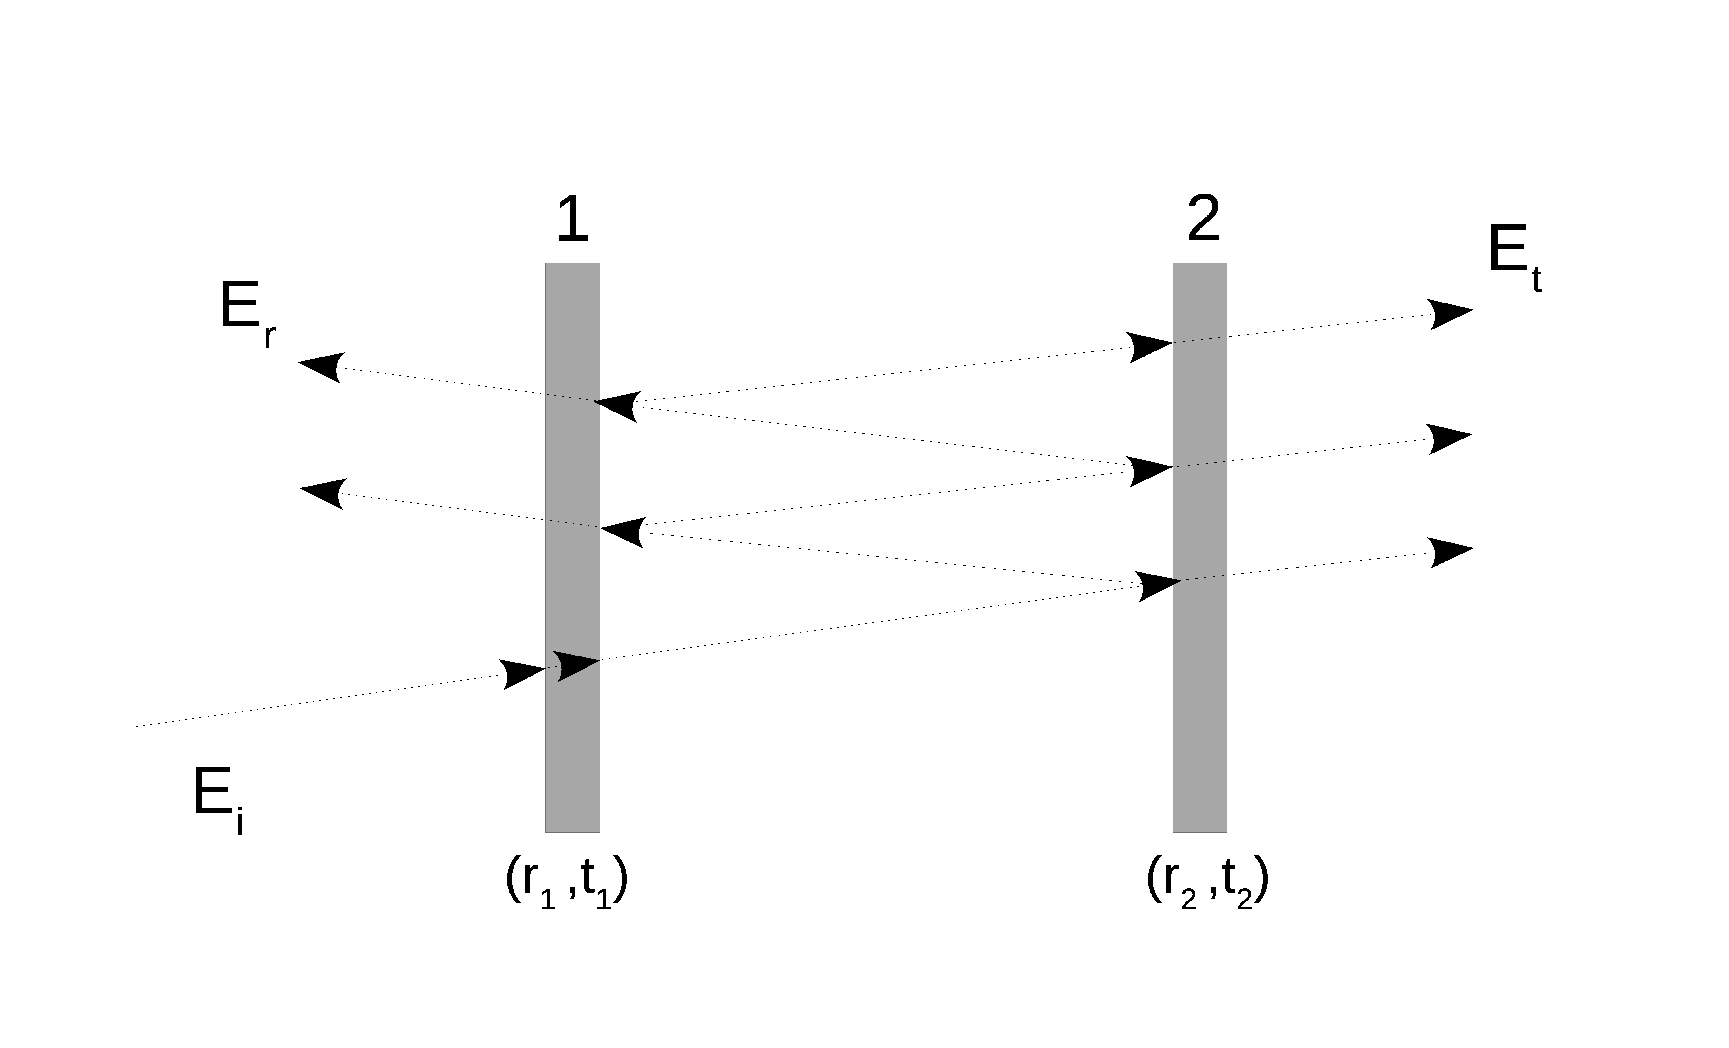
\includegraphics[width=0.65\textwidth]{Fabry_Perot_resonator.eps}
\caption{Illustrated energy diagram of a simple Fabry-Perot resonator}
\end{figure}

\newpage

\subsection{Theory of Fabry-Perot interferometer}
 If the incident energy is in the form of white coherent light then at that point the transmission and reflection coefficients depend just on the mirror reflectivities. The total reflected power comprises of the power reflected from the principal mirror in addition to all the different reflections between the mirrors that add to the reflectivity in general. In summation, the equations are: 
\begin{equation}
{\mathcal R} = R_{1} + T_{1}^2 R_{2} \sum_{m=1}^{\infty} (R_{1}R_{2})^{m-1} = \frac{R_{1} - 2R_{1}R_{2} + R_{2}}{1 - R_{1}R_{2}} _{\overrightarrow{R_{1} = R_{2} \equiv R}} \frac{2R}{1+R}
\end{equation}

Similarly, the transmitted energy in summation is:
\begin{equation}
{\mathcal T} = T_{1} T_{2} \sum_{m=1}^{\infty} (R_{1}R_{2})^{m-1} = \frac{T_{1} T_{2}}{1 - R_{1}R_{2}} _{\; \overrightarrow{R_{1} = R_{2} \equiv R}} \; \frac{T^{2}}{1-R^{2}} = \frac{1-R}{1+R}
\end{equation}

Assuming, be that as it may, the incident light comprises of a transiently lucid (monochromatic) plane wave, at that point the reflected power will be relative to the square of the reasonable total of every reflected field. Since the fields convey phase information with amplitudes added, the division of reflected and transmitted light depends not just on the mirror reflectivities, but in addition on the mirror separation and excitation wavelength. The rational 

total of fields is amplified when every one of the fields interfere constructively (in phase) and limited when they interfere destructively (out of phase). 

Phase gathers with propogation separation as $\phi(z) = \beta z$ and may likewise be gained upon communication with the mirrors. The sound forms of 

Eqs. 2.1 and 2.2 incorporate an aggregated stage factor for each round-trip that can be translated as a standardized detuning $\phi = T_{R}\omega$, where $T_{R}$ is the cavity travel time, $T_{R} = n_{eff}L/c$ for the circumference, L and effective index $n_{eff}$. Presently, $\tilde{r}$ speaks to the complex reflectivity:

\begin{multline}
\tilde{r} = r_{1} - t_{1}^{2}r_{2}\exp{(i m \phi)} \sum_{m=1}^{\infty} (r_{1}r_{2}\exp{(i m \phi)})^{m-1} \\ = \frac{r_{1} - r_{2}\exp{(i \phi)}}{1 - r_{1}r_{2}\exp{(i \phi)}} _{\; \overrightarrow{r_{1} = r_{2} \equiv r}} \; \frac{r(1-\exp{(+i \phi)})}{1-r^{2}\exp{(+i \phi)}}
\end{multline}

and $\tilde{t}$ represents the complex transmittivity:

\begin{multline}
\tilde{t} = -t_{1}t_{2}\exp{(i m \phi/2)} \sum_{m=1}^{\infty} (r_{1}r_{2}\exp{(i m \phi)})^{m-1} \\ = \frac{-t_{1}t_{2}\exp{(i m \phi/2)}}{1 - r_{1}r_{2}} _{\; \overrightarrow{r_{1} = r_{2} \equiv r}} \; \frac{-(1-r^{2})\exp{(im \phi/2)}}{1-r^{2}}
\end{multline}


The square modulus of these perplexing amounts gives the reflection ${\mathcal R}$ and transmission ${\mathcal T}$ coefficients. Antiresonant wavelengths are more emphatically reflected than in the ambiguous case, while thunderous wavelengths are transmitted $100\%$ for adjusted reflectors ($r_{1}$ = $r_{2}$). For a fixed reflect dispersing, the transmission and reflection spectra in this manner show intermittent pinnacles and valleys. Figure 3.1 presenting the transmission and reflection spectra for a lossless, adjusted Fabry– Perot resonator. The part of reflected and transmitted power for mixed up excitation is identical to the separate frightfully arrived at the midpoint of reflection and transmission over a time of the spectrum range.
\subsection{Finese, Q-factor}
\subparagraph{\normalfont \large To perform more advanced calculations, it is important to have some understanding of how mpmath works internally and what the possible sources of error are. This section gives an overview of arbitrary-precision binary floating-point arithmetic and some concepts from numerical analysis.Most of the time, using mpmath is simply a matter of setting the desired precision and entering a formula. For verification purposes, a quite (but not always!) reliable technique is to calculate the same thing a second time at a higher precision and verifying that the results agree.}
\section{Gain incorporation in Resonators}
To perform more advanced calculations, it is important to have some understanding of how mpmath works internally and what the possible sources of error are. This section gives an overview of arbitrary-precision
\subsection{Beer's Law}
 binary floating-point arithmetic and some concepts from numerical analysis.Most of the time, using mpmath is simply a matter of setting the desired precision and entering a formula. For verification purposes, a quite (but not always!) reliable technique is to calculate the same thing a second time at a higher precision and verifying that the results agree.
\subsection{Beer's law study as gain}
To perform more advanced calculations, it is important to have some understanding of how mpmath works internally and what the possible sources of error are. This section gives an overview of arbitrary-precision binary floating-point arithmetic and some concepts from numerical analysis.Most of the time, using mpmath is simply a matter of setting the desired precision and entering a formula. For verification purposes, a quite (but not always!) reliable technique is to calculate the same thing a second time at a higher precision and verifying that the results agree.
\section{Gain medium}
To perform more advanced calculations, it is important to have some understanding of how mpmath works internally and what the possible sources of error are. This section gives an overview of arbitrary-precision binary floating-point arithmetic and some concepts from numerical analysis.